%
%
%
%

\section{Background} \label{sec:background}

\subsection{Persistent Homology}
Persistent homology, the flagship tool from the field of Topological Data Analysis (TDA), is used to measure the shape of a dataset at multiple dimensions. For example, it can measure connected components (dimension zero), loops (dimension one), voids (dimension two), and higher dimensional analogues. 
Persistent homology measures these shapes using a parameterized filtration to detect when the structures are born (appear) and die (disappear). 
We give the basic ideas in this section and direct the interested reader to more complete introductions to 
standard homology \cite{Hatcher,Munkres2}
and persistent homology \cite{Dey2021,Oudot2015,Munch2017}.

The required input for persistence is a filtration of a simplicial complex $K$. 
Specifically,  a filtration $\{K_{a_i}\}_i$ is a parameterized sequence of simplicial complexes which are nested; i.e.
\begin{equation}
K_{\alpha_0} \subseteq K_{\alpha_1} \subseteq K_{\alpha_2} \subseteq \ldots \subseteq K_{\alpha_n}.
\label{eq:nested_complexes}
\end{equation}
Under this notation, there are $n+1$ simplicial complexes; and it is often the case that $K_{\alpha_0}$ is either the empty complex or the complex consisting of only the vertex set. 
We can then calculate the homology of dimension $p$ for each complex, $H_p(K_{a_i})$, which is a vector space representing the $p$-dimensional structure of the space such as loops, voids, etc.
Surprisingly, there is further information to be used, namely that the inclusions on the simplicial complexes induce linear maps on the vector spaces resulting in a construction called a persistence module: 
\begin{equation}
H_p(K_{\alpha_0}) \to H_p(K_{\alpha_1}) \to H_p(K_{\alpha_2}) \to \ldots \to H_p(K_{\alpha_n}).
\label{eq:filtration}
\end{equation}

The appearance and disappearance of classes in this object can be tracked, resulting in a representation of the information known as a persistence diagram. 
For each class which appears at $K_{b_i}$ and disappears at $K_{d_i}$, we draw a point in the plane at $(b_i,d_i)$. 
Taken together, the collection of points (also called persistence pairs), all of which are above the diagonal $\Delta= \{ (x,y) \mid x = y\}$, is called a persistence diagram. 



One common approach to obtain this setup is in the case where the input data is a finite metric space $(M,d)$; i.e.~a finite set $M$ with distances given by $d(m_1,m_2)$. 
For example, $M$ might be a finite point cloud $\chi \subset \R^k$ with $d$ given by Euclidean distance. 
In the case of a graph $G$ as input data, we can have $M=V$ the vertex set, and $d(u,v)$ as the number of edges in the shortest path between vertex $u$ and vertex $v$. 

From this metric space data, we fix a value $\alpha \geq 0$ and construct the Vietoris-Rips (VR) complex, denoted $R_\alpha(M)$. 
In the VR construction, we have a vertex set $M$ and a simplex $\sigma \subseteq M$ is included in the abstract simplicial complex $R_\alpha(M)$ whenever $d(v,w) \leq \alpha$ for all $v,w \in \sigma$. 
Then by definition, $R_\alpha(\chi) \subseteq R_{\alpha'}(\chi)$ whenever $\alpha \leq \alpha'$. 
In this particular context, the axes of the persistence diagram correspond to distances between points.
So, for example, points in the diagram that are far from the diagonal of the 1-dimensional persistence diagram represent large loop structures in the input data. 

\begin{figure}
    \centering
    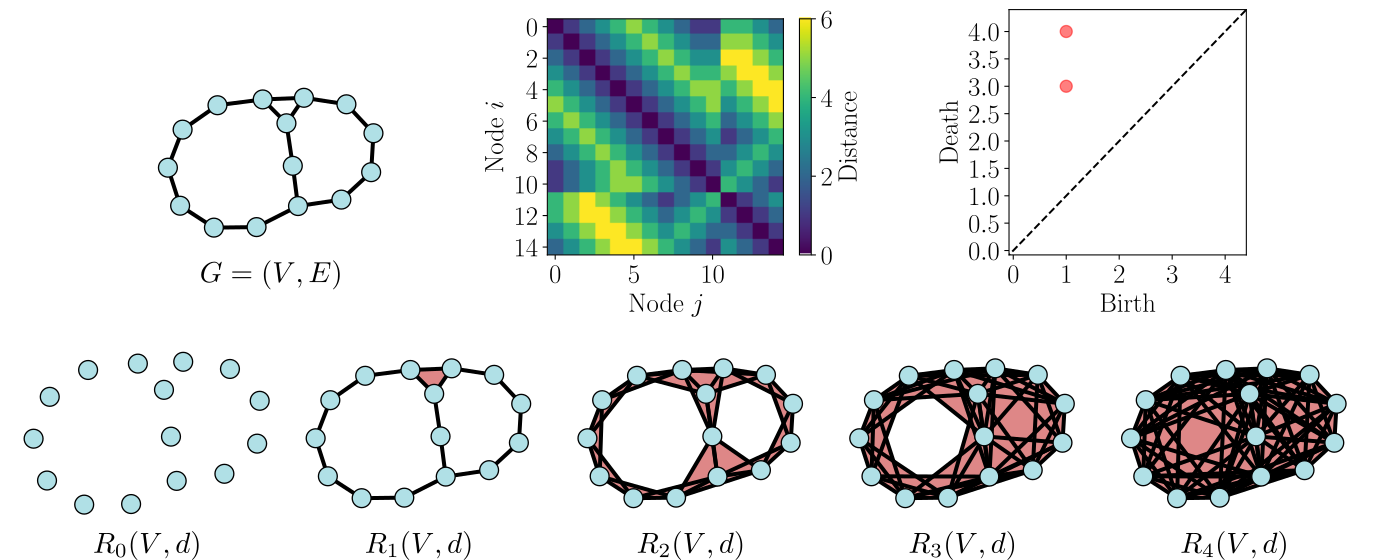
\includegraphics[width = \textwidth]{Figures/BigExampleFig-StandardPers.png}
    \caption{An example of a Rips filtration where the input is the shortest path distance on an example graph $G$. The persistence diagram in the top right is for standard persistence rather than zigzag as will be discussed later in the paper. }
    \label{fig:bigGraphPersistence}
\end{figure}
See Fig.~\ref{fig:bigGraphPersistence} for an example of the filtration in this setting. 
The graph $G$ is shown at the top left, and the distance defined on the nodes is given in the matrix at the top middle. 
The bottom row shows the Rips complexes for different choices of $\alpha$ parameter. 
In particular, note that $R_1(V,d)$ has the graph $G$ as the 1-skeleton, but includes an additional triangle not present in the graph. 
The top right shows the 1-dimensional persistence diagram. 
Note that the two large loops in the graph are encoded as points in the diagram; while the small triangle is immediately filled in and thus not represented. 


%

\subsection{Zigzag Persistence}

%
%
%
%
%
%
%
%
%
%
%
%
%
%
%
%
%
%
%
%
%
%
%
%
%
%
%
%
%
%
%
%
%
%
%
%
%
%


A limitation of the standard setup of persistent homology is that it requires each simplicial complex to be a subset of the next, as shown in Eq.~\eqref{eq:nested_complexes}.
This means that at each step, we are only allowed to add new simplices to the previous complex to build this filtration. 
However, temporal graphs have no such behavior.
%
%
Thus, this issue can be alleviated through zigzag persistence~\cite{Carlsson2010, Carlsson2009a}, which allows for inclusions which can go either way at each step. 
This is often written as 
\begin{equation}
K_{\alpha_0} \leftrightarrow K_{\alpha_1} \leftrightarrow K_{\alpha_2} \leftrightarrow \ldots \leftrightarrow K_{\alpha_n},
\label{eq:bi_directional_zigzag_complexes}
\end{equation}
where $\leftrightarrow$ denotes one of the two inclusions $\hookrightarrow$ and $\hookleftarrow$. 

A common special case of this definition is where the left and right inclusions alternate, which can arise by taking a sequence of simplicial complexes, and interleaving them with either unions or intersections of the adjacent complexes.
Focusing on the case of the union, denote $K_{i,i+1} = K_i \cup K_{i+1}$ to get the zigzag filtration
\begin{equation*}
K_{\alpha_0} \hookrightarrow K_{\alpha_0,\alpha_1} 
\hookleftarrow K_{\alpha_1} 
\hookrightarrow K_{\alpha_1,\alpha_2} 
\hookleftarrow K_{\alpha_2} 
\hookrightarrow \ldots 
\hookleftarrow K_{\alpha_{n-1}}  
\hookrightarrow K_{\alpha_{n-1},\alpha_{n}} 
\hookleftarrow K_{\alpha_n}.
%
\end{equation*}
%

%




The same algebra that makes it possible for standard persistence to be represented in a diagram allows for computation of when homology features are born and die based on the zigzag persistence, however one must take care as some of the intuition from standard persistence is lost.
We can again track this with a persistence diagram consisting of persistence pairs $(b_i, d_i)$. 
In the case of a class appearing or disappearing at the union complex $K_{\alpha_{i},\alpha_{i+1}}$, we draw the index at the average $(\alpha_i+\alpha_{i+1})/2$.
If a topological feature persists through the last simplicial complex we set its death as the end time of the last window or index $n+0.5$. 
%


\begin{figure}%
    \centering
    
\includegraphics[width=0.83\textwidth]{simple_zigzag_example}
    \caption{
    %
    Example application of zigzag persistence to study changing topology of simplicial complex sequence. This example shows the sequence of simplicial complexes with intermediate unions and corresponding time stamps on the left and on the right the resulting zigzag persistence diagram on the right for dimension $0$ and $1$ as $H_0$ and $H_1$, respectively.
    %
    }
    \label{fig:simple_zigzag_example}
\end{figure}
To demonstrate how zigzag persistence tracks the changing topology in a sequence of simplicial complexes we will use a simple example shown in Fig.~\ref{fig:simple_zigzag_example}. 
The sequence of simplicial complexes are shown as $[K_{0}, K_{1}, K_{2}]$, with unions given by 
$K_{0,1}$ and $K_{1,2}$.
The persistence diagram then tracks where topological features of various dimensions of $H_p$ (dimension 0 and 1 for this example) form and disappear. 
For example, for $H_0$ there are two components in $K_{0}$. 
At the next simplicial complex $K_{0,1}$ the two $0$-dimensional features combine signifying one of their deaths which is tracked in the persistence diagram as the persistence pair $(0,0.5)$ since 0.5 is the average of $0$ and $1$. 
The component that persists remains throughout all of the simplicial complexes. 
Therefore, we set its death as the last time stamp plus 0.5 and record the persistence pair as $(0, 2.5)$. 
On the other hand, there is a single loop (a 1-dimensional feature) which is shown only at $K_{0,1}$. 
For technical reasons, this is drawn as a point with birth time 0.5 (the average of $0$ and $1$) and death time 1 since it dies entering $K_{1}$. 

\begin{figure}%
    \centering
    \begin{minipage}{0.21\textwidth}
         \centering
         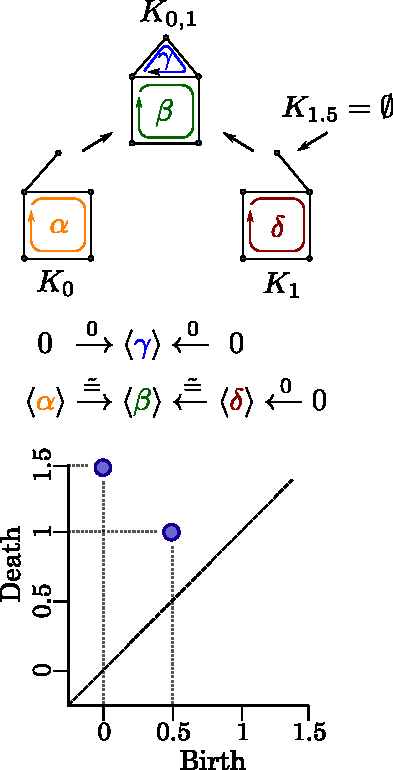
\includegraphics[width=\textwidth]{Figures/case1_zigzag_issue} \\
         (a) Case 1
         %
         %
    \end{minipage}
    \hfill
    \begin{minipage}{0.21\textwidth}
         \centering
         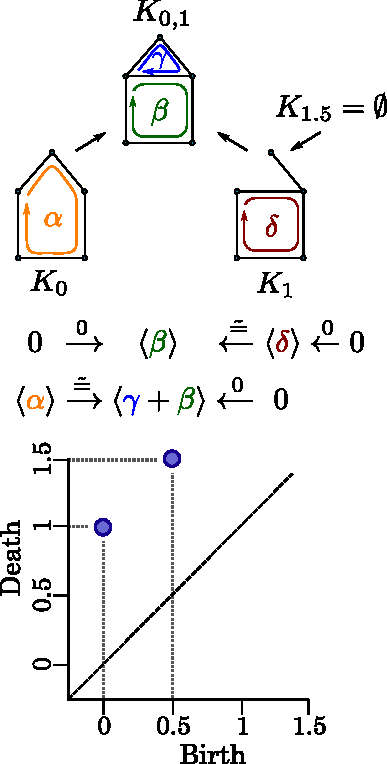
\includegraphics[width=\textwidth]{Figures/case2_zigzag_issue} \\
         (b) Case 2
         %
         %
    \end{minipage}
    \hfill
    \begin{minipage}{0.21\textwidth}
         \centering
         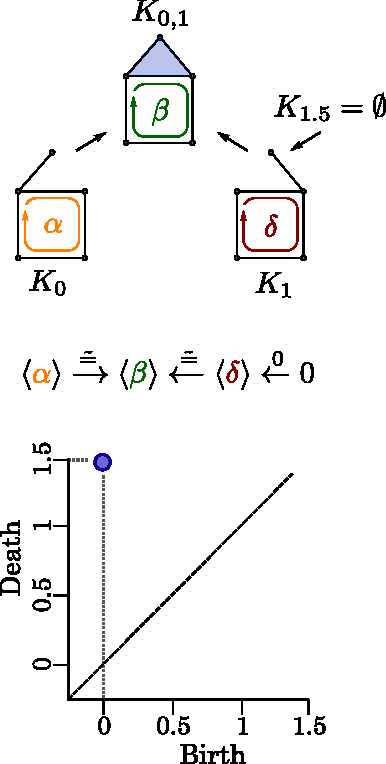
\includegraphics[width=\textwidth]{Figures/case3_zigzag_issue} \\
         (c) Case 3
         %
         %
    \end{minipage}
    \hfill
    \begin{minipage}{0.21\textwidth}
         \centering
         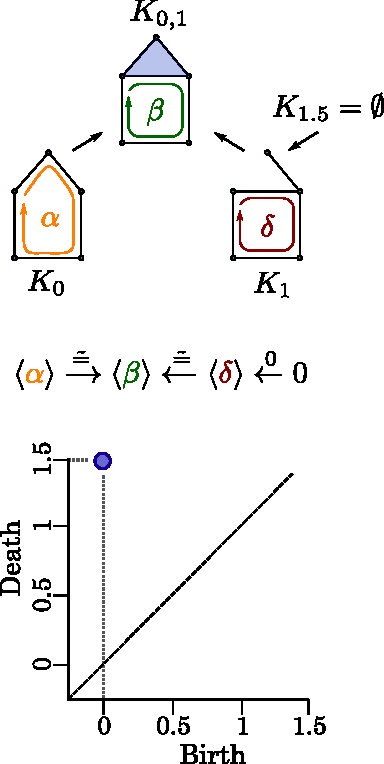
\includegraphics[width=\textwidth]{Figures/case4_zigzag_issue} \\
         (d) Case 4
         %
         %
    \end{minipage}
    \caption{Several examples showing how the zigzag persistence diagram can be affected by the existence of small loops. 
    The first and third; and the second and fourth examples have the same filtration with the addition of a single triangle in the later case. 
    In each case, the generators of homology are shown with the interval decomposition drawn below. The resulting persistence diagrams show that the third and fourth examples show a single bar representing the persisting loop. 
    However in the first two intervals are quite different, where the long lived bar is split into two pieces in the second example.
    %
    }
    \label{fig:HouseExample}
\end{figure}
It should be noted that sometimes zigzag persistence results are counter-intuitive to those used to standard persistence interpretation.  
For example, consider the example of Fig.~\ref{fig:HouseExample}.
The first two filtrations each appear to have a circular structure which lasts through the duration of the filtration, however, the zigzag persistence diagram sees the first case as a class living throughout, while the second breaks this class into two individual bars. 
In this case at least, the issue can be mitigated by including a triangle at the top of the house filling in the short cycle, resulting in both filtrations having only a single point in the persistence diagram representing the loop in the house. 

Secondly, we also note that the axes in the zigzag diagram correspond to indexing in the zigzag diagram.  
This means that a point far from the diagonal means there is a loop structure that is present for a large portion of the index set, rather than being a measurement of size of that same loop. 


